\documentclass[12pt]{article}
\usepackage[utf8]{inputenc}
\usepackage{sbc-template}

\usepackage{graphicx,url}

%\usepackage[brazil]{babel}   


     
\sloppy

\title{Segurança para a Internet das Coisas: Uma Solução para Comunicação Criptografada entre Dispositivos}

\author{Erik Henrique de Oliveira Zambeli - RA: 1749927}


\address{Universidade Tecnológica Federal do Paraná (UTFPR)\\
  Campus Cornélio Procópio -- PR -- Brazil
}

\begin{document} 

\maketitle

\begin{abstract}
  resumo..
\end{abstract}
     
\begin{resumo} 
  resumo..
\end{resumo}


\section{Introdução}

% \begin{figure}[ht]
% \centering
% \includegraphics[width=.5\textwidth]{fig1.jpg}
% \caption{A typical figure}
% \label{fig:exampleFig1}
% \end{figure}

\section{Referencial Teórico}

Criptografia é uma palavra grega formada pela junção dos termos Kryptos e Grapho (grafia, escrita). Ela utiliza uma sequência de passos que servem para transformar um texto claro em texto codificado que aparenta ser um texto gerado aleatoriamente sem possuir sentido algum. A ação de transformar dados para uma forma ilegível é denominada cifra ou cifragem, e busca garantir  a  privacidade. O processo inverso da cifragem é chamado de decifragem. Quando utilizamos o processo de cifragem e decifragem, necessitamos de informações confidenciais, chamadas chaves \cite{STALLINGS:14}. Existem dois tipos de chaves:

Chave Simétrica: É também conhecida como criptografia de chave privada. O emissor usa uma chave para cifrar a mensagem, e o receptor utiliza a mesma chave para decifrá-la. 

Chave Assimétrica: Conhecida como  criptografia de  chave  pública. Este tipo de  criptografia,  usamos  duas  chaves  distintas,  de  modo  a  obtermos  comunicação  segura através de canais de comunicação inseguros. Trata-se de uma técnica de criptografia assimétrica pelo fato de usar um par de chaves distintos.

\subsection{Algoritmos criptográficos}

Os algoritmos criptográficos podem ser implementados em hardware (para performance) ou software (para flexibilidade), mais a maior parte do tratamento esta relacionado aos algoritmos e protocolos, que são independentes da implementação real \cite{TANENBAUM:03}.Podemos dizer que um algoritmo de criptografia é um procedimento matemático que contém uma entrada (dados a serem cifrados), efetua um processamento matemático com base em uma chave, e gera uma saída.

\subsubsection{Criptografia Simétrica}


A criptografia simétrica é conhecida por criptografia de chave secreta. Este modelo usa uma única chave que é partilhada entre o emissor e o receptor figura, \ref{cripto1}. Desta forma, a chave que é usada para cifrar é a mesma que é usada para decifrar. Quando  uma pessoa  quer  se  comunicar  de  forma  segura  com  outra  pessoa, as maquinas já devem conhecer a chave secreta ou a chave utilizada para cifrar a mensagem deve ser enviada pela rede. Este processo é chamado de “distribuição de chaves”. Algoritmos que usam criptografia simétrica tendem a ser mais rápidos, no entanto não são tão seguros, uma vez que a chave usada para cifrar a informação é partilhada entre as várias máquinas da rede. A maior dificuldade do método é a distribuição segura das chaves\cite{BURNETT:02}.

 \begin{figure}[h!]
	\centering
	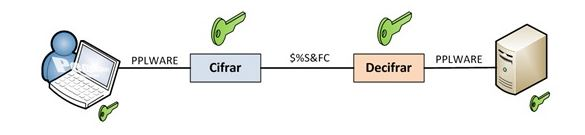
\includegraphics[]{Simetrica.JPG}
	\caption{Funcionamento Criptografia Simétrica}
	\label{cripto1}
\end{figure}

\subsubsection{Algoritmos de Criptografia Simétrica}
    Os algoritmos  DES , 3DES e AES são alguns dos que utilizam a criptografia simétrica. Podemos analisar outros algoritmos  de  chave  privada  ou  criptografia  simétrica  de  forma  resumida  na Tabela \ref{tab1}:
\begin{table}[h!]
\caption{Principais algoritmos de chave privada ou criptografia simétrica}
\label{tab1}
\begin{tabular}{|l|l|l|}
\hline
Algoritmo & Bits                                                     & Descrição                                                                                                                                           \\ \hline
AES       & 128                                                      & \begin{tabular}[c]{@{}l@{}}O Advanced Encryption Standard (AES) é uma cifra de bloco, \\ anunciado pelo National Institute of Standards and Technology (NIST) \\ em  2003,  fruto  de  concurso  para  escolha  de  um  novo algoritmo  \\ de  chave  simétrica  para  proteger  informações  do governo federal, \\ sendo adotado como padrão pelo governo dos Estados  Unidos,  é  \\ um  dos  algoritmos  mais  populares,  desde 2006, usado   para   \\ criptografia   de   chave   simétrica,   sendo considerado como o \\ padrão substituto do DES. O AES tem um tamanho de bloco fixo em \\ 128 bits e uma chave com tamanho de 128, 192 ou 256 bits, ele é \\ rápido tanto em software quanto em hardware, é relativamente fácil \\ de executar e requer pouca memória.\end{tabular} \\ \hline
DES       & 56                                                       & \begin{tabular}[c]{@{}l@{}}O  Data  Encryption  Standard  (DES)  foi  o  algoritmo  simétrico mais  \\ disseminado  no mundo,  até  a  padronização  do  AES.  Foi criado  \\ pela  IBM  em  1977  e,  apesar  de  permitir  cerca  de  72 quadrilhões \\ de combinações, seu tamanho de chave (56 bits) é considerado pequeno, \\ tendo sido quebrado por "força bruta" em 1997 em um desafio lançado na \\ Internet. O NIST que lançou o desafio  mencionado,  recertificou  o  DES  \\ pela  última  vez  em 1993, passando então a recomendar o 3DES.\end{tabular} \\ \hline   \end{tabular}  
\end{table}

\begin{table}[h!]
\begin{tabular}{|l|l|l|}
\hline
3DES      & \begin{tabular}[c]{@{}l@{}}112 \\ ou \\ 168\end{tabular} & \begin{tabular}[c]{@{}l@{}}O 3DES é uma simples variação do DES, utilizando o em três ciframentos  \\ suscessivos,  podendo  empregar  uma  versão  com duas ou com três \\ chaves diferentes. É seguro, porém muito lento para ser um algoritmo \\ padrão.\end{tabular}                                                                                                                                                                                                                                                                                                                                                                                                                                                                                                                       \\ \hline
IDEA      & 128                                                      & \begin{tabular}[c]{@{}l@{}}O  International Data Encryption Algorithm (IDEA) foi  criado em  1991  \\ por  James  Massey  e  Xuejia  Lai  e  possui  patente  da suíça  ASCOM  \\ Systec.  O  algoritmo  é  estruturado  seguindo  as mesmas linhas  gerais do \\ DES. Mas    na   maioria    dos microprocessadores,  uma   implementação  \\ por   software   do IDEA  é  mais  rápida  do  que  uma  implementação  por  \\ software do  DES.  O  IDEA  é  utilizado  principalmente  no  mercado \\ financeiro  e  no  PGP,  o  programa  para  criptografia  de  e-mail pessoal \\ mais disseminado no mundo.\end{tabular}                                                                                                                                                                \\ \hline
\end{tabular}
\centering Fonte:\cite{STALLINGS:14}
\end{table}




\subsubsection{Criptografia Assimétrica}

A  criptografia assimétrica,conhecida  por  criptografia de  chaves  públicas, faz p  uso  de  pares  de  chaves  para criptografar ou descriptografar. As duas chaves  são  relacionadas  através  de  um  processo  matemático, usando  funções  unidirecionais para a codificação da informação. A chave pública que, como o nome já diz, qualquer um pode conhecer e ter acesso, é usada para cifrar, enquanto a chave privada, é usada para decifrar. Uma mensagem cifrada com uma chave pública somente poderá ser decifrada com o uso da chave privada com a qual está  relacionada. O método  traz segurança, pois não é necessário compartilhar a chave privada. Em contrapartida, o tempo de processamento de mensagens com criptografia assimétrica é muito maior do que com criptografia simétrica \cite{BURNETT:02}. 
Na Figura \ref{cripto2} é demonstrado o processo.

 \begin{figure}[h!]
	\centering
	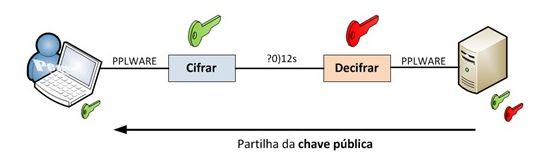
\includegraphics[]{assimetrica.JPG}
	\caption{Funcionamento Criptografia assimétrica}
	\label{cripto2}
\end{figure}

\subsubsection{Algoritmos de Criptografia Assimétrica}

A grande dificuldade deste sistema é a  complexidade  no  desenvolvimento  dos algoritmos que devem reconhecer a dupla de chaves existentes e relacionar as  mesmas  no  momento  certo,  o  que reverte num  grande  poder  de  processamento computacional para este trabalho \cite{STALLINGS:14}. A  analise  dos  principais  algoritmos  de  chave pública ou criptografia assimétrica de forma resumida na Tabela \ref{tab2}.

\begin{table}[h!]
\caption{Principais algoritmos de chaves públicas ou criptografia assimétrica}
\label{tab2}
\begin{tabular}{|l|l|}
\hline
Algoritmo                                                  & Descrição                                                                                                                                                                                                                                                                                                                                                                                                                                                                                                                                                                                                                                                                                                                                                                                                                                                                                                                                                                                                                                                                                                                                                                                                                                                                                                                                                                                                                                                                                                                                                                                                                                                                                                                                                                                                                                                                                                                                                                              \\ \hline
RSA                                                        & \begin{tabular}[c]{@{}l@{}}O RSA  é  um algoritmo  assimétrico  que  possui  este  nome  devido  a  seus \\ inventores:  Ron  Rivest,  Adi Shamir  e  Len  Adleman,  que  o  criaram  em \\ 1977   no   MIT.   Atualmente,   é   o   algoritmo   de   chave   pública   mais \\ amplamente  utilizado,  além  de  ser  uma  das  mais  poderosas  formas  de \\ criptografia  de  chave  pública  conhecidas  até  o  momento.  O  RSA  utiliza \\ números  primos.  A  premissa  por  trás  do  RSA  consiste  na  facilidade  de \\ multiplicar dois números primos para obter um terceiro número, mas muito \\ difícil de recuperar os dois primos a partir daquele terceiro número. Isto é \\ conhecido como fatoração. Por exemplo, os fatores primos de 3.337 são 47 \\ e  71.  Gerar  a  chave  pública  envolve  multiplicar  dois  primos  grandes; \\ qualquer  um  pode  fazer  isto.  Derivar  a  chave  privada  a  partir  da  chave \\ pública  envolve  fatorar  um  grande  número.  Se  o  número  for  grande  o \\ suficiente  e  bem  escolhido,  então  ninguém  pode  fazer  isto  em  uma \\ quantidade  de  tempo  razoável.  Assim,  a  segurança  do  RSA  baseia  se  na \\ dificuldade  de  fatoração  de  números  grandes.  Deste  modo,  a  fatoração \\ representa   um   limite   superior   do   tempo   necessário   para   quebrar   o \\ algoritmo. Uma chave RSA de 512 bits foi quebrada em 1999 pelo Instituto \\ Nacional  de  Pesquisa  da  Holanda,  com  o  apoio  de  cientistas  de  mais  6 \\ países. Levou cerca de 7 meses e foram utilizadas 300 estações de trabalho \\ para a quebra. No Brasil, o RSA é utilizado pela ICP-Brasil, no seu sistema \\ de emissão de certificados digitais, e a partir do dia 1º de janeiro de 2012, \\ as  chaves  utilizadas  pelas  autoridades  certificadoras  do  país,  passam  a \\ serem  emitidas  com  o  comprimento  de  4.096bits,  em  vez  dos  2.048bits \\ atuais.\end{tabular} \\ \hline
ElGamal                                                    & \begin{tabular}[c]{@{}l@{}}O   El Gamal   é   outro   algoritmo   de   chave   pública   utilizado   para \\ gerenciamento de chaves. Sua matemática difere da utilizada no RSA, mas \\ também  é  um  sistema  comutativo.  O  algoritmo  envolve  a  manipulação \\ matemática  de  grandes  quantidades  numéricas.  Sua  segurança  advém  \\ de algo  denominado  problema  do  logaritmo  discreto.  Assim,  o  ElGamal \\ obtém sua segurança da dificuldade de calcular logaritmos discretos em um \\ corpo finito, o que lembra bastante o problema da fatoração.\end{tabular}                                                                                                                                                                                                                                                                                                                                                                                                                                                                                                                                                                                                                                                                                                                                                                                                                                                                                                                                                                                                                                                                                                                                                                                                                                                                                                                                                                                                \\ \hline
\begin{tabular}[c]{@{}l@{}}Diffie -\\ Hellman\end{tabular} & \begin{tabular}[c]{@{}l@{}}Também baseado no problema do logaritmo discreto, e o criptosistema de \\ chave pública mais antigo ainda em uso. O conceito de chave pública, aliás \\ foi  introduzido  pelos  autores  deste  criptosistema em 1976.  Contudo,  ele \\ não permite nem ciframento nem assinatura digital. O sistema foi projetado \\ para permitir a dois indivíduos entrarem em um acordo ao compartilharem \\ um  segredo  tal  como  uma  chave,  muito  embora  eles  somente  troquem \\ mensagens em público.\end{tabular}                                                                                                                                                                                                                                                                                                                                                                                                                                                                                                                                                                                                                                                                                                                                                                                                                                                                                                                                                                                                                                                                                                                                                                                                                                                                                                                                                                                                                                         \\ \hline
\end{tabular}
\centering Fonte: \cite{STALLINGS:14}
\end{table}

\section{Aplicação}
% CRIPTOGRAFIA SIMÉTRICA – utiliza apenas uma chave. Esta chave é utilizada tanto para criptografar quanto para descriptografar a mensagem.
% CRIPTOGRAFIA ASSIMÉTRICA – Utiliza duas chaves. Uma pública e outra privada. A mensagem criptografada por uma chave publica só pode ser descriptografada por uma chave privada correspondente.

the author names references in brackets, e.g. \cite{knuth:84},
 and \cite{smith:99}.

\bibliographystyle{sbc}
\bibliography{sbc-template}

\end{document}
